\section{Rezultate benzi circulație}

Aplicația are o precizie în detecție a benzilor de circulație pe video-urile analizate de $92.3\%$ detecții corecte și o rată de detecții false de $8.75\%$. Rezultatele detalitate pot fi vizualizate în tabelul 4.1.

\begin{table}[h!]
	\centering
	\begin{tabular}{||c | c | c | c | c | c ||} 
		\hline
		Video & Total frame-uri & Total linii & Detectații & Detecții corecte & Detecții false \\ [0.5ex] 
		\hline\hline
		cordova1 & 250 & 449 & 467 & 91.31\% & 12.69\%  \\ 
		washington1 & 336 & 667 & 662 & 88.48\% & 9.31\% \\
		washington2 & 232 & 448 & 454 & 97.10\% & 4.24\%  \\ 
		\hline\hline
		Total & 818 & 1 564 & 1 583 & 92.30\% & 8.75\% \\ [1ex]
		
		\hline
	\end{tabular}
	\caption{Rezultate evaluare detecție bandă}
	\label{table:1}
\end{table}

În continuare pot fi vizualizate diverse exemple reușite, în figura 4.2, iar altele mai puțin reușite, în figura 4.3.

\begin{figure}[!h]
	\centering
	\includegraphics[max width=15cm,max height=15cm,keepaspectratio]{img_4_2}
	\caption[Detecție bandă - exemple reușite]{Exemple reușite. Rând 1 - cordova1, 2 - washington1, 3 - washington2.}
\end{figure}
\begin{figure}[!h]
	\centering
	\includegraphics[max width=15cm,max height=15cm,keepaspectratio]{img_4_3}
	\caption[Detecție bandă - exemple nereușite]{Exemple nereușite. Rând 1 - cordova1, 2 - washington1, 3 - washington2.}
\end{figure}

\section{Bază de date benzi circulație}
\subsection*{Informații generale}

Partea din aplicație ce are rolul de a detecta banda curentă de circulație a fost dezvoltat plecând de la baza de date Caltech Lanes Dataset de imagini.  \hyperlink{Bazadedatebenzidecirculatie}{[4]}

\subsection*{Tipuri de imagini}

Caltech Lanes Dataset conține $1225$ de imagini cu adnotările de rigoare. Baza de date este împărțită în patru tipuri de clipuri și anume: $cordova1$ cu un număr total de 250 de imagini, $cordova2$ cu un număr total de 406 de imagini, $washington1$ cu un număr total de 337 de imagini și $washington2$ cu un număr total de 232 de imagini. Dintre aceste patru seturi de imagini au fost folosite cordova1, washington1 și washington2.

\begin{figure}[!h]
	\centering
	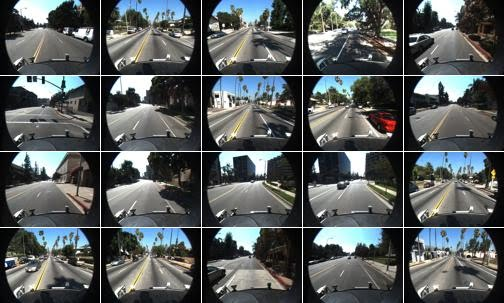
\includegraphics[max width=15cm,max height=15cm,keepaspectratio]{img_4_1}
	\caption[Imagini Caltech Lanes Dataset]{Exemple imagini din baza de date Caltech Lanes Dataset.}
\end{figure} 

\subsection*{Algoritm de evaluare}

Pentru evaluarea rezultatelor a fost folosit soft-ul de evaluare propus de autorul articolului Real time Detection of Lane Markers in Urban Streets \hyperlink{MohamedAly}{[11]}. 
Asupra acestuia au fost aduse modificări în privința citirii etichetelor asociate fiecărui video. Astfel, în cazul lucrării de față, accentul se pune pe banda curentă de circulație. Pentru a extrage doar aceste etichete au fost selectate conform distanței acestora față de centrul imaginii cu o încadrare într-un interval definit în prealabil.

\section{Rezultate detecție mașină}

Precizia medie obțiuntă de aplicație este de 91.30\% după cum se poate observa în figura 4.4.

\begin{figure}[!h]
	\centering
	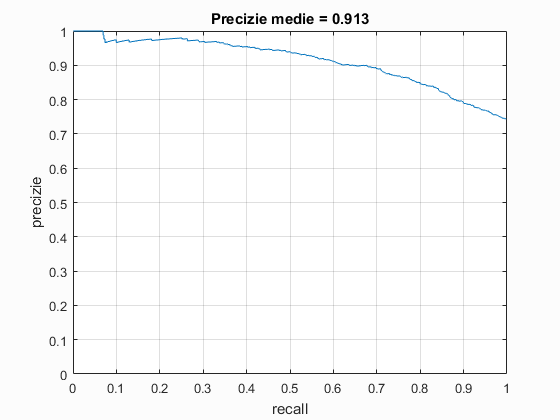
\includegraphics[max width=11cm,max height=11cm,keepaspectratio]{img_4_4}
	\caption{Grafic precizie - recall detecție mașină}
\end{figure}

În figura 4.5 și 4.6 sunt prezentate exemple reușite și exemple nereușite. 

\begin{figure}[!h]
	\centering
	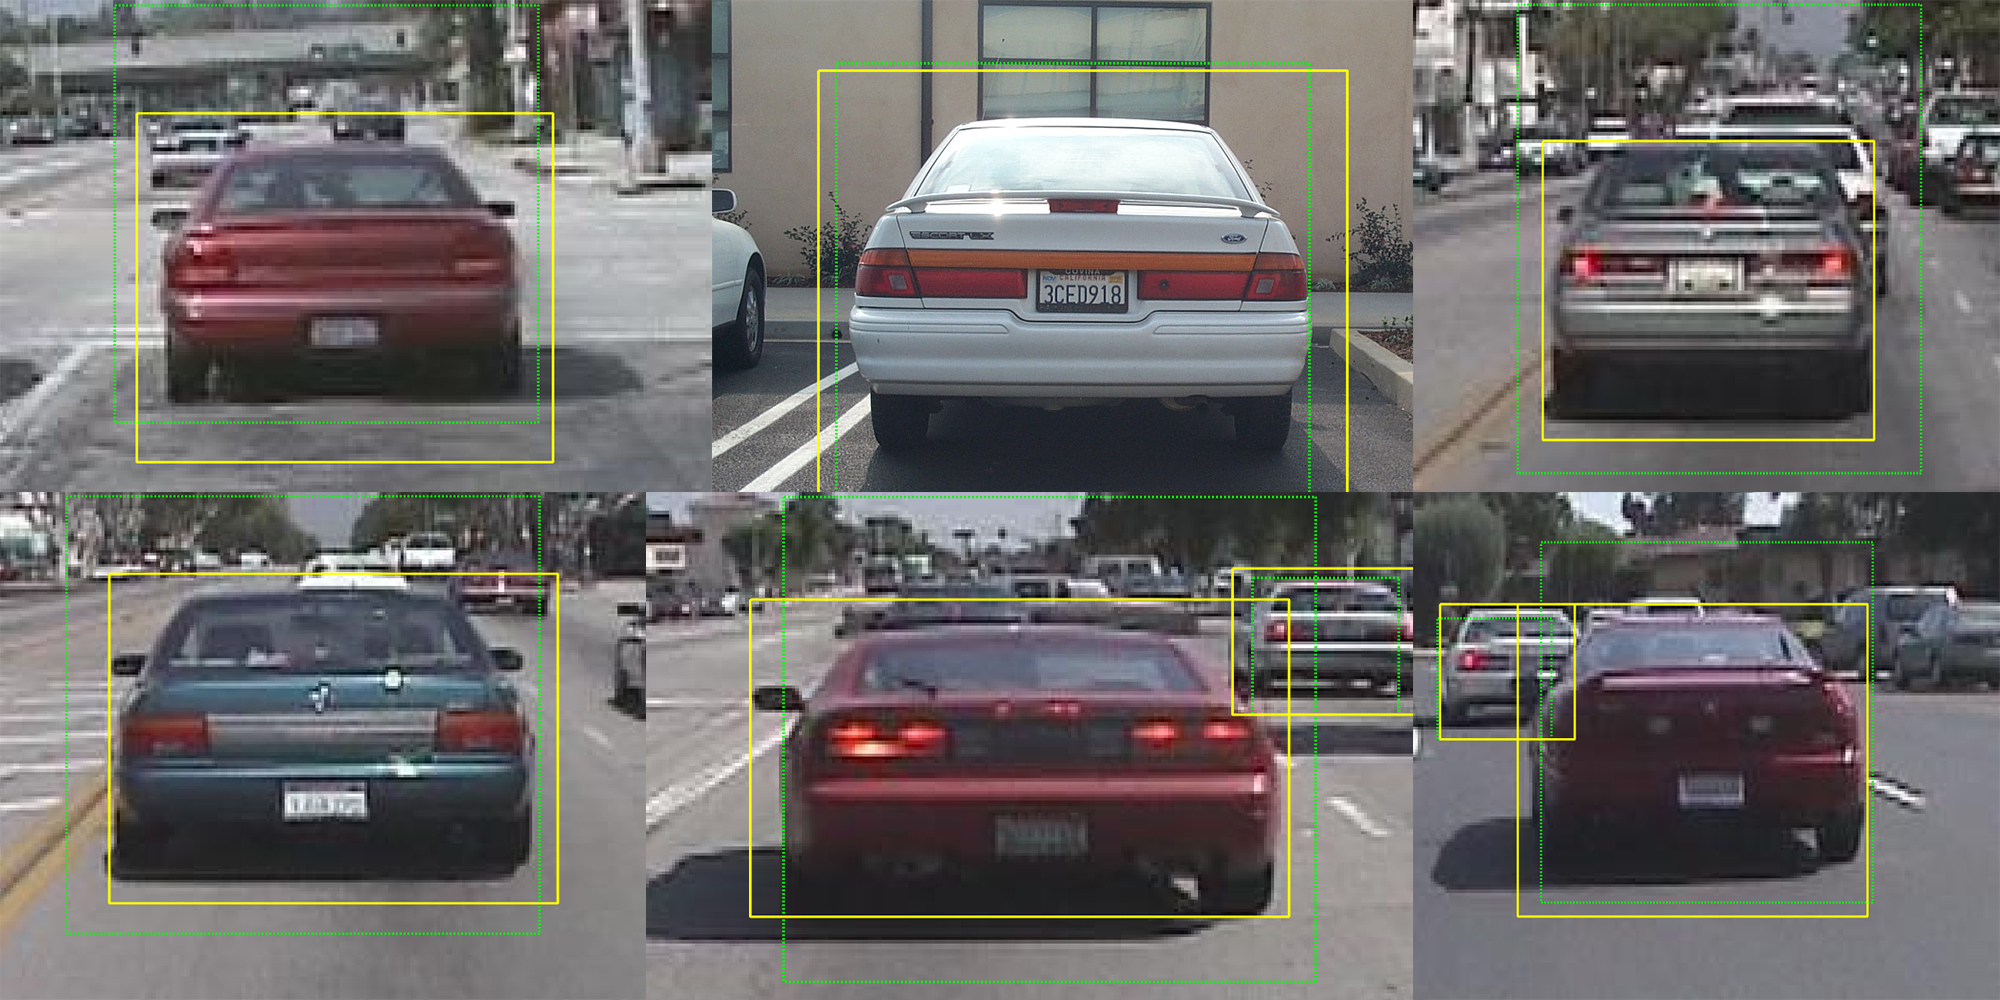
\includegraphics[max width=11cm,max height=11cm,keepaspectratio]{img_4_5}
	\caption{Detecție mașini - exemple reușite}
\end{figure}
\begin{figure}[!ht]
	\centering
	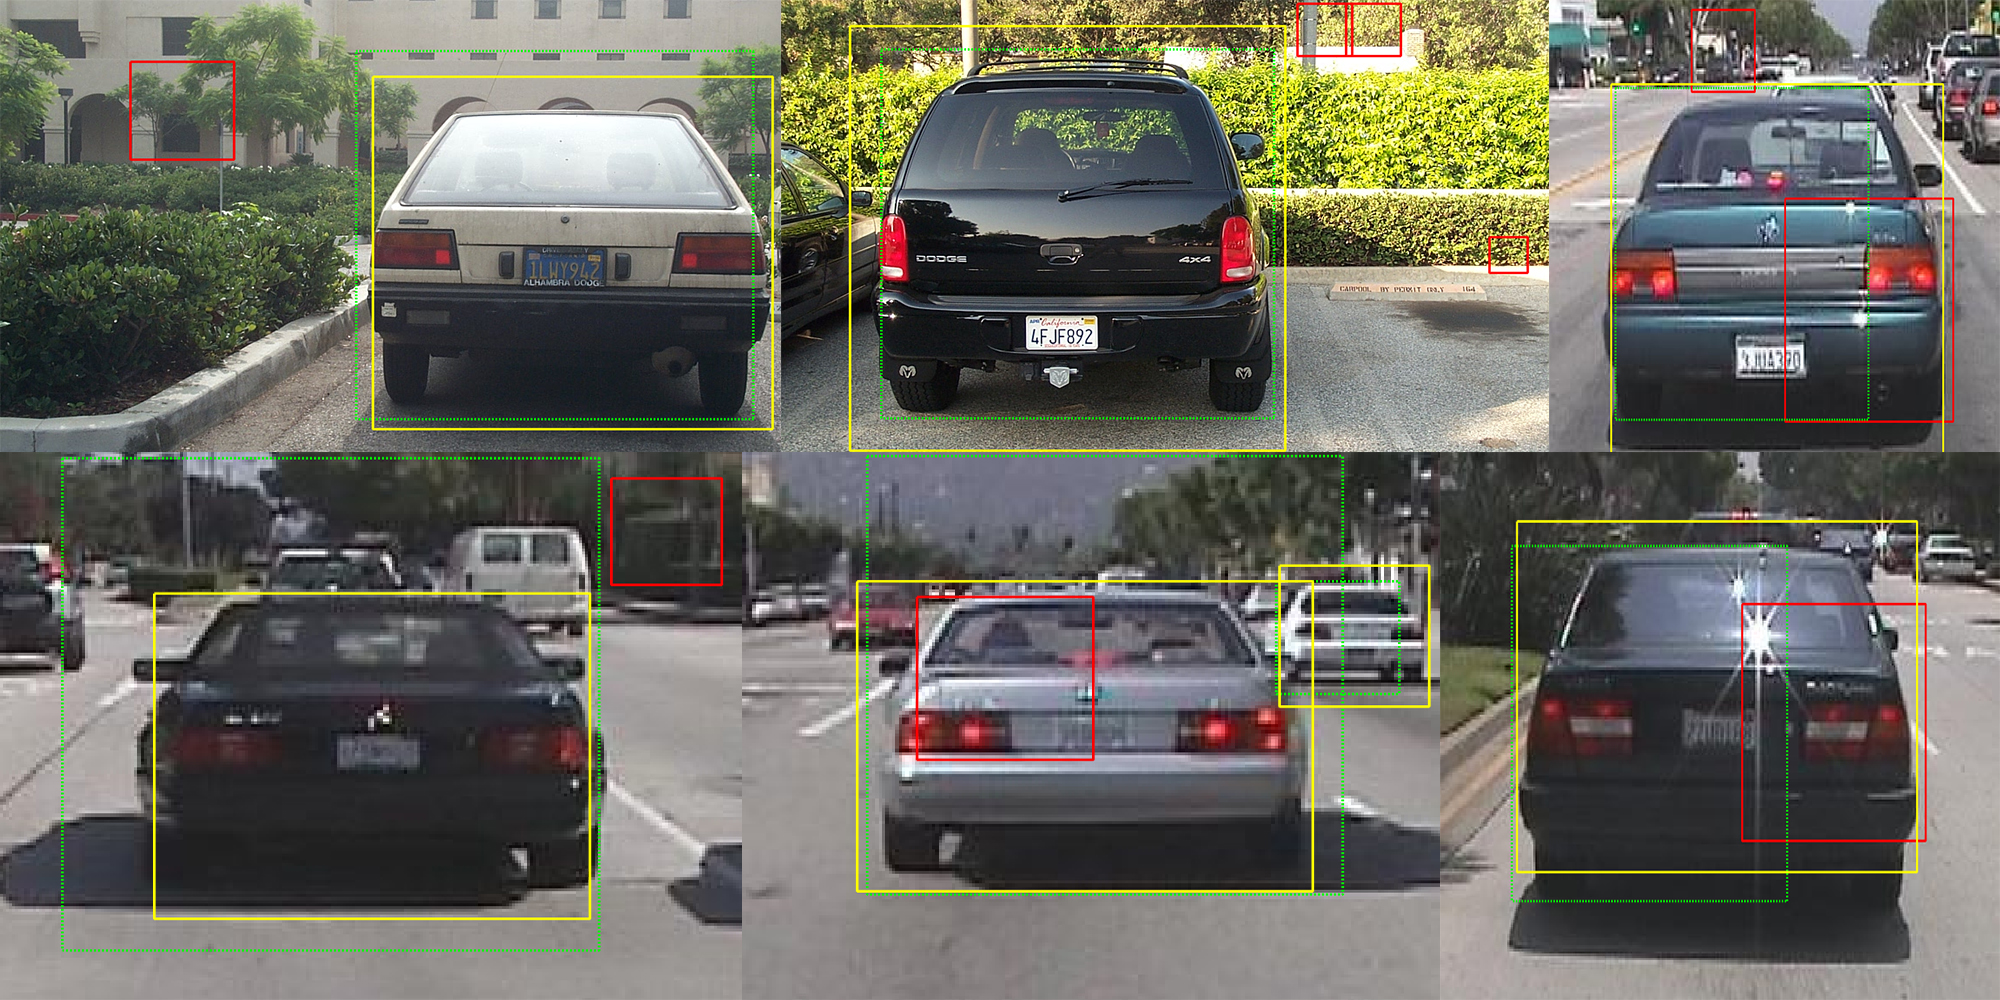
\includegraphics[max width=11cm,max height=11cm,keepaspectratio]{img_4_6}
	\caption{Detecție mașini - exemple nereușite}
\end{figure}

\section{Bază de date mașini}

\subsection*{Informații generale}

În cazul componentei ce se ocupă de detectarea mașinii au fost folosite două baze de date. Prima dintre aceasta, cea oferită de Universitatea Politehnică din Madrid și a fost folosită pentru antrenarea clasificatorilor \hyperlink{BazadedatemasiniUniversitateaPolitehnicadinMadrid}{[3]}.

Pentru testarea a fost folosită o altă bază de date cu imagini, oferită de Universitatea Oxford ce vine în completarea bazei de date oferite de Institutul de Tehnologie din California \hyperlink{BazadedatemasiniUniversitateaOxford}{[2}, \hyperlink{BazadedatemasiniInstituluideTehnologiedinCalifornia}{5]}.

\subsection*{Tipuri de imagini}

Baza de date oferită de Universitatea Politehnică din Madrid cuprinde două tipuri principale de imagini. Prima categorie conține imagini cu mașini și este împărțită în alte patru subcategori: mașini fotografiate din stânga, mașini fotografiate din dreapta, mașini fotografiate din depărtare și mașini fotografiate din centru. Aceste patru subcategori însumează un număr total de 3 425 de imagini. Aceste imagini provin din diferite condiții, spre exemplu imagini din vreme însorită, înorată, condiții medii, ploaie, iluminat artificial sau iluminare slabă.

A doua parte a acestei baze de date este reprezentată de imaginile de antrenare negative, ce nu conțin mașini. La rândul lor sunt împărțite în cele patru subcategori menționate anterior și însumează un număr total de 3 900 de imagini.

Baza oferită de Universitatea Oxford este formată la rândul ei din alte două baze de date de imagini. Aceste imagini nu au venit insoțite de etichete, astfel etichetarea a fost făcută ulterior. Din contopirea celor 2 baze de date a rezultat un set de 987 de imagini cu mașini pentru testare.

\subsection*{Algoritm de evaluare}

În ceea ce privește algoritmul de evaluare, fiecare fereastră ce poate conține o mașină oferită de aplicație a fost comparată cu etichetele asociate imaginii respective, iar dacă suprapunere dintre locația indicată de aplicație și locația etichetată se află într-un anumit prag predefinit este acceptată ca detecție adevărată, în caz contrar, este clasificată ca fiind o detecție falsă.